\subsection{Desain Kelas Batasan Tabu}\label{desain_kelas_tabu}
Kelas batasan tabu digunakan untuk memudahkan penyimpanan data tabu berupa jumlah langkah, batasan tabu, dan aksi yang dibatasi tabu. Kelas ini memiliki dua metode yaitu memilih aksi dan mengecek kebolehan aksi. Desain kelas batasan tabu dapat dilihat pada Gambar \ref{fig:class_tabuLimit}.

\begin{figure}[ht]
	\centering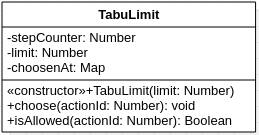
\includegraphics[width=0.5\textwidth]{bab3/figures/class_tabuLimit.png}
	\caption{Desain kelas batasan tabu}
	\label{fig:class_tabuLimit}
\end{figure}

\subsubsection{Desain Konstruktor Batasan Tabu}
Konstruktor untuk kelas batasan tabu berfungsi untuk menginisialisasi nilai batasan dan jumlah langkah awal agar kelas ini dapat digunakan. \textit{Pseudocode} dari konstruktor kelas batasan tabu dapat dilihat pada Gambar \ref{psdo:tabu_constructor}.

\begin{figure}[ht]
	\begin{lstlisting}[firstnumber=0]
	TabuLimit(limit)
	this->limit = limit
	this->stepCounter = limit + 1
	\end{lstlisting}
	\caption{\textit{Pseudocode} konstruktor kelas batasan tabu}
	\label{psdo:tabu_constructor}
\end{figure}

\subsubsection{Desain Metode Memilih Aksi}
Metode ini berfungsi untuk mencatat langkah saat aksi tersebut dilakukan, selanjutnya nilai langkah akan ditambah. \textit{Pseudocode} untuk metode ini dapat dilihat pada Gambar \ref{psdo:tabu_choose}.

\begin{figure}[ht]
	\begin{lstlisting}[firstnumber=0]
	choose(actionId: Number): void
	choosenAt[actionId] = this->stepCounter
	this->stepCounter++
	\end{lstlisting}
	\caption{\textit{Pseudocode} metode memilih aksi}
	\label{psdo:tabu_choose}
\end{figure}

\subsubsection{Desain Mengecek Kebolehan Aksi}
Metode ini mengecek kebolehan suatu aksi dengan cara menghitung selisih dari nilai langkah sekarang dengan langkah saat aksi tersebut dipilih, jika selisihnya kurang dari limit maka aksi tersebut dibolehkan. \textit{Pseudocode} dari metode ini dapat dilihat pada Gambar \ref{psdo:tabu_isAllowed}.

\begin{figure}[ht]
	\begin{lstlisting}[firstnumber=0]
	isAllowed(actionId: Number): Boolean
	stepDifference = this->stepCounter - this->choosenAt[actionId]
	return (stepCounter > this->limit)
	\end{lstlisting}
	\caption{\textit{Pseudocode} metode mengecek kebolehan aksi}
	\label{psdo:tabu_isAllowed}
\end{figure}